\documentclass[a4paper]{article}
\usepackage[swedish]{babel}
\usepackage[margin=2.5cm]{geometry}
\usepackage[T1]{fontenc}
\usepackage[utf8]{inputenc}

\pagenumbering{roman}

\usepackage{tabularx}

\usepackage[dvipsnames]{xcolor}
\usepackage{listings}
\lstset{
	language=c++,
	basicstyle=\ttfamily,
	keywordstyle=\bfseries\color{red},
	commentstyle=\itshape\color{ForestGreen},
	identifierstyle=\color{blue},
    stringstyle=\color{orange},
	numbers=left,
	frame=single,
	captionpos =b,
	breaklines=true
	escapeinside=`',
	escapebegin={\color{editorGray}}
	}
		
\usepackage{graphicx}
\graphicspath{ {../Drawings/} }

\begin{document}
\title{
	\textbf{Othellobot}\\
	\textit{Elektromekaniskt projekt (5hp)}
}
\author{Jacob Olofsson, Thomas Danielsson, Aksel Wännström}
\maketitle

\pagebreak

\begin{abstract}
Denna rapport beskriver ett konstruktionsprojekt med mål att konstruera en robot som kan spela brädspelet Othello (även kallat reversi) mot en mänsklig spelare.
Pjäserna konstruerades i plast med en permanentmagnet inuti.
Hall-sensorer monterades sedan i spelplanen för att kunna läsa av ifall rutorna i spelplanen var tomma, innehöll svarta pjäser eller vita pjäser.
Ett AI baserat på en Monte Carlo-algoritm beräknar sedan det bästa möjliga draget.
Detta drag utförs sedan med en robotarm som flyttar sig längs en bana ovanför spelplanen som håller den magnetiska spelpjäsen med hjälp av en elektromagnet.
\end{abstract}

\tableofcontents

\pagebreak
\pagenumbering{arabic}

\section{Introduktion}
\subsection{Othello}
Spelet \textit{Reversi} uppfanns på 1880-talet i london och har sedan dess spritt sig runt hela världen.
Idag är spelet mer känt vid namnet \textit{Othello}.

\subsubsection*{Spelregler}
Spelet spelas av två spelare, hädanefter svart och vit.
Spelplanen är normalt ett bräde indelat i 8x8 rutor men kan spelas med ett mindre eller större antal rutor.
Spelpjäserna är svarta på ena sidan och vita på den andra.
Sidan som ligger uppåt visar vilken spelare pjäsen hör till.
Spelet startar med fyra pjäser, två från varje spelare i mitten i ett schackmönster.
Spelarna turas om att placera ut en pjäs i taget i ett tomt fält.
När en pjäs placeras ut ska alla av motspelarens pjäser som ligger i raka linjer (horisontella, vertikala eller diagonala) mellan den utplacerade pjäsen och en annan pjäs av den spelande spelaren vändas.
Ett drag är endast tillåtet om minst en av motståndarens pjäser vänds av draget.
Ifall det inte finns några möjliga drag måste spelaren passa sin tur tills det finns ett möjligt drag att göra.
När ingen kan göra några fler drag är spelet slut och den spelare med mest pjäser på brädet vinner.

\subsection{Mål}
Målet med detta projekt är att att konstruera en robot och ett AI som kan spela Othello mot en mänsklig motståndare.
AI:t ska kunna hämta tillräckligt med information för att göra ett drag som är tillåtet enligt spelets regler.

\section{Teori}
För att en robot ska kunna spela Othello måste den på något sätt kunna läsa av spelplanen, tänka fram ett bra drag och sedan fysiskt utföra draget.

\subsection{Sensorer}
För att kunna läsa av spelbrädet finns det många tillvägagångssätt.
Eftersom en robot som ska spela othello måste veta om varje ruta på spelplanen antingen är tom, har en svart spelpjäs eller en vit spelpjäs på sig finns det 3 olika tillstånd för varje ruta.
För detta ändamål lämpar sig någon form av linjär sensor som kan läsas av analogt bra.
Sensorer kan då sättas vid varje ruta på spelplanen och kalibreras så att de är mättade åt ena hållet för en svart pjäs,  mättade åt andra hållet för en vit pjäs och någonstans mitt emellan när rutan är tom.

\subsection{AI-algoritm} \label{AI}
Ett vanligt sätt att bygga ett AI för att spela ett spel är att på något sätt bygga ett beslutsträd där alla möjliga dra utvärderas.
Denna sorts algoritm växer exponentiellt i både tids- och minneskomplexitet vilket gör att den inte lämpar sig särskilt bra för en resursbegränsad plattform som t.ex. en mikrokontroller.
Därför har vi valt att använda oss av en Monte Carlo-metod.
Monte Carlo-metoden går ut på att istället för att bygga ett stort träd simuleras spel utifrån den nuvarande uppställningen på planen med slumpmässiga drag.
Programmet håller räkningen på vinster och förluster och väljer sedan det drag som i genomsnitt lett till flest vinster bland de slumpade spelen.
Denna algoritm använder en konstant minneskomplexitet och kommer att ge ett bättre svar desto längre den får tänka men betänketiden går att anpassa exakt efter omständigheterna.
Algoritmen kan sammanfattas i följande steg:
\begin{itemize}
\item Hämta alla möjliga drag
\item Medan tidsbegränsningen inte gått ut: 
	\begin{itemize} 
	\item Välj nästa möjliga drag
	\item Utför draget och starta simulering
	\item Medan simuleringen (spelet) inte är över:
		\begin{itemize}
		\item Byt spelare
		\item Gör slumpmässigt drag
		\end{itemize}	
	\item Spara vinst/förlust
	\end{itemize}
\item Välj det drag som gett mest vinster i medelvärde
\end{itemize}

\subsection{Robotarm}
För att roboten ska kunna plocka upp en pjäs och sedan släppa den på rätt plats på spelplanen behövs tre frihetsgrader.
Armen behöver kunna röra sig tvärsöver planen (två dimensioner) samt lyfta och sänka en pjäs den håller i.
Rörelserna kan dock vara ganska begränsade då roboten endast behöver komma åt ett antal fördefinierade rutor och inget utanför det (förutom att plocka upp en ny pjäs).
Rörelsen i höjdled kan vara ännu mer begränsad, den behöver egentligen vara binär.
Antingen är den i höjd för att plocka upp en spelpjäs eller så är den i höjd för att kunna flytta spelpjäsen ovanför de andra pjäserna.

\section{Metod}
\subsection{Mjukvara}
Designen av mjukvaran är indelad i fem stycken moduler som ansvarar för sin egen del av designen och en toppnivå som knyter samman modulerna, se figur \ref{system_arch}.
Se appendix \ref{code} för fullständig kod.
\begin{figure}\label{system_arch}
\centering
\includegraphics[scale=0.6]{system_arch}
\caption{Den implementerade mjukvaruarkitekturen. Huvudmodulen \texttt{othello\_bot} kommunicerar med de andra undermodulerna. Det gemensamma interfacet \texttt{game} är sättet modulerna kommunicerar med varandra.}
\end{figure}

\subsubsection*{game}
Modulen \texttt{game} implementerar spelreglerna och definierar spelbrädet.
Modulen definierar även koordinaterna till spelbrädet och vad en spelare är.
Den här modulen har ingen kontakt med hårdvaran.

\subsubsection*{AI}
Modulen \texttt{AI} implementerar AI:t som beskrivts i del \ref{AI}.
Modulen tar ett state i form av ett spel och en spelarfärg som definieras i modulen \texttt{game} och beräknar det bästa draget.

\subsubsection*{move\_planner}
Modulen \texttt{move\_planner} ansvarar för att ta ett drag (i form av en spelare och en koordinat) och sedan utföra det fysiskt.
Det är den här modulen som har kontakt med hårdvaran för styrning.

\subsubsection*{IO}
Modulen \texttt{IO} ansvarar för att kommunicera med hårdvaran, att läsa av knappar för att programmet ska veta om de kan börja på nästa tur och skriva information om programmets status till LEDs.

\subsubsection*{sensor}
Modulen \texttt{sensor} ansvarar för att läsa av sensorerna i spelbrädet samt att tolka detta till en representation av spelbrädet som definierats i \texttt{game}.
Den här modulen har också direkt kontakt med hårdvaran.

\subsection{Hårdvara}
Som kontroller till projektet valdes en Arduino för att hålla komplexiteten i programmeringen nere.
Vidare valdes en Arduino Mega för att ha tillgång till så många analoga portar som möjligt för sensorerna samt att ha så mycket processorkraft som möjligt för AI:t.
Som linjära sensorer valdes Hall-sensorer och spelpjäserna konstruerades med magneter inuti.
Detta medförde att en elektromagnet blev ett passande val för att plocka upp och släppa pjäser.
Elektromagneten sattes på en två-dimensionell bana likt en 3D-skrivare och drivs med två stegmotorer (via kugghjul och kuggremmar) för precision.
Elektromagneten kan sedan sänkas eller höjas med ett servo.
Se ritningar i appendix \ref{sketches} för mer detaljer.

\section{Resultat}
\subsection{Konstruktion}
\subsubsection*{Ställning}
Förflyttningen skapades genom att bygga en ställning av metallstängerstänger.
Vinkellister sågades av och användes för att ställningar som höll ihop dessa metallstänger och även agera som plattform för att sätta fast elektromagnet, servo och stegmotor på mittenplattan.
Styrningen skapades genom att koppla ihop två metallstänger på var sin sida om ställningen där ena var kopplad till en stegmotor.
Detta kan ses i figur \ref{board_uppe}.
Ställningen kunde röra sig till viss del men på grund av friktion i ställningen orkade inte stegmotorerna att röra sig hela vägen till ändpunkterna.
Därigenom kunde endast 8stycken spelpjäser nås i nuvarande konfiguration.
\begin{figure}\label{board_uppe}
\centering
\includegraphics[width=\textwidth,keepaspectratio]{../images/board_uppe}
\caption{Toppsidan av ställningen med spelplan under. Mitten ses elektromagentställningen med stegmotor för ena ledden. Andra ledden styrs av en stegmotor precis utanför bild ner till vänster.}
\end{figure}

\subsubsection*{Elektromagnet}
Elektromagneten gjordes av en spik som lindades med koppartråd.
Då denna måste kunna vända polaritet beroende på vilken sida av magneten som är uppåt samt även slås av och på så var planen att koppla in en två stycken relän som i konfigurationen som ses i figur xx.
Att just relän användes var på grund av att Arduinon inte kan leverera tillräckligt mycket ström för att producera tillräckligt kraftigt magnetfält utan en extern strömförsöjning måste utnyttjas.
Denna elektromagnet måste kunna lyftas upp ovanför resterade spelpjäser för att inte påverka dessa med magneterna.
Detta genomfördes med ett servo som med hjälp av att linda upp en tråd kan höja elektromagneten, ses i figur \ref{servo_fram}.
Elektromagneten testades och kunde uppnå önskat resultat, dock har inte lösningen med relän implementerats ännu.
\begin{figure}\label{servo_fram}
\centering
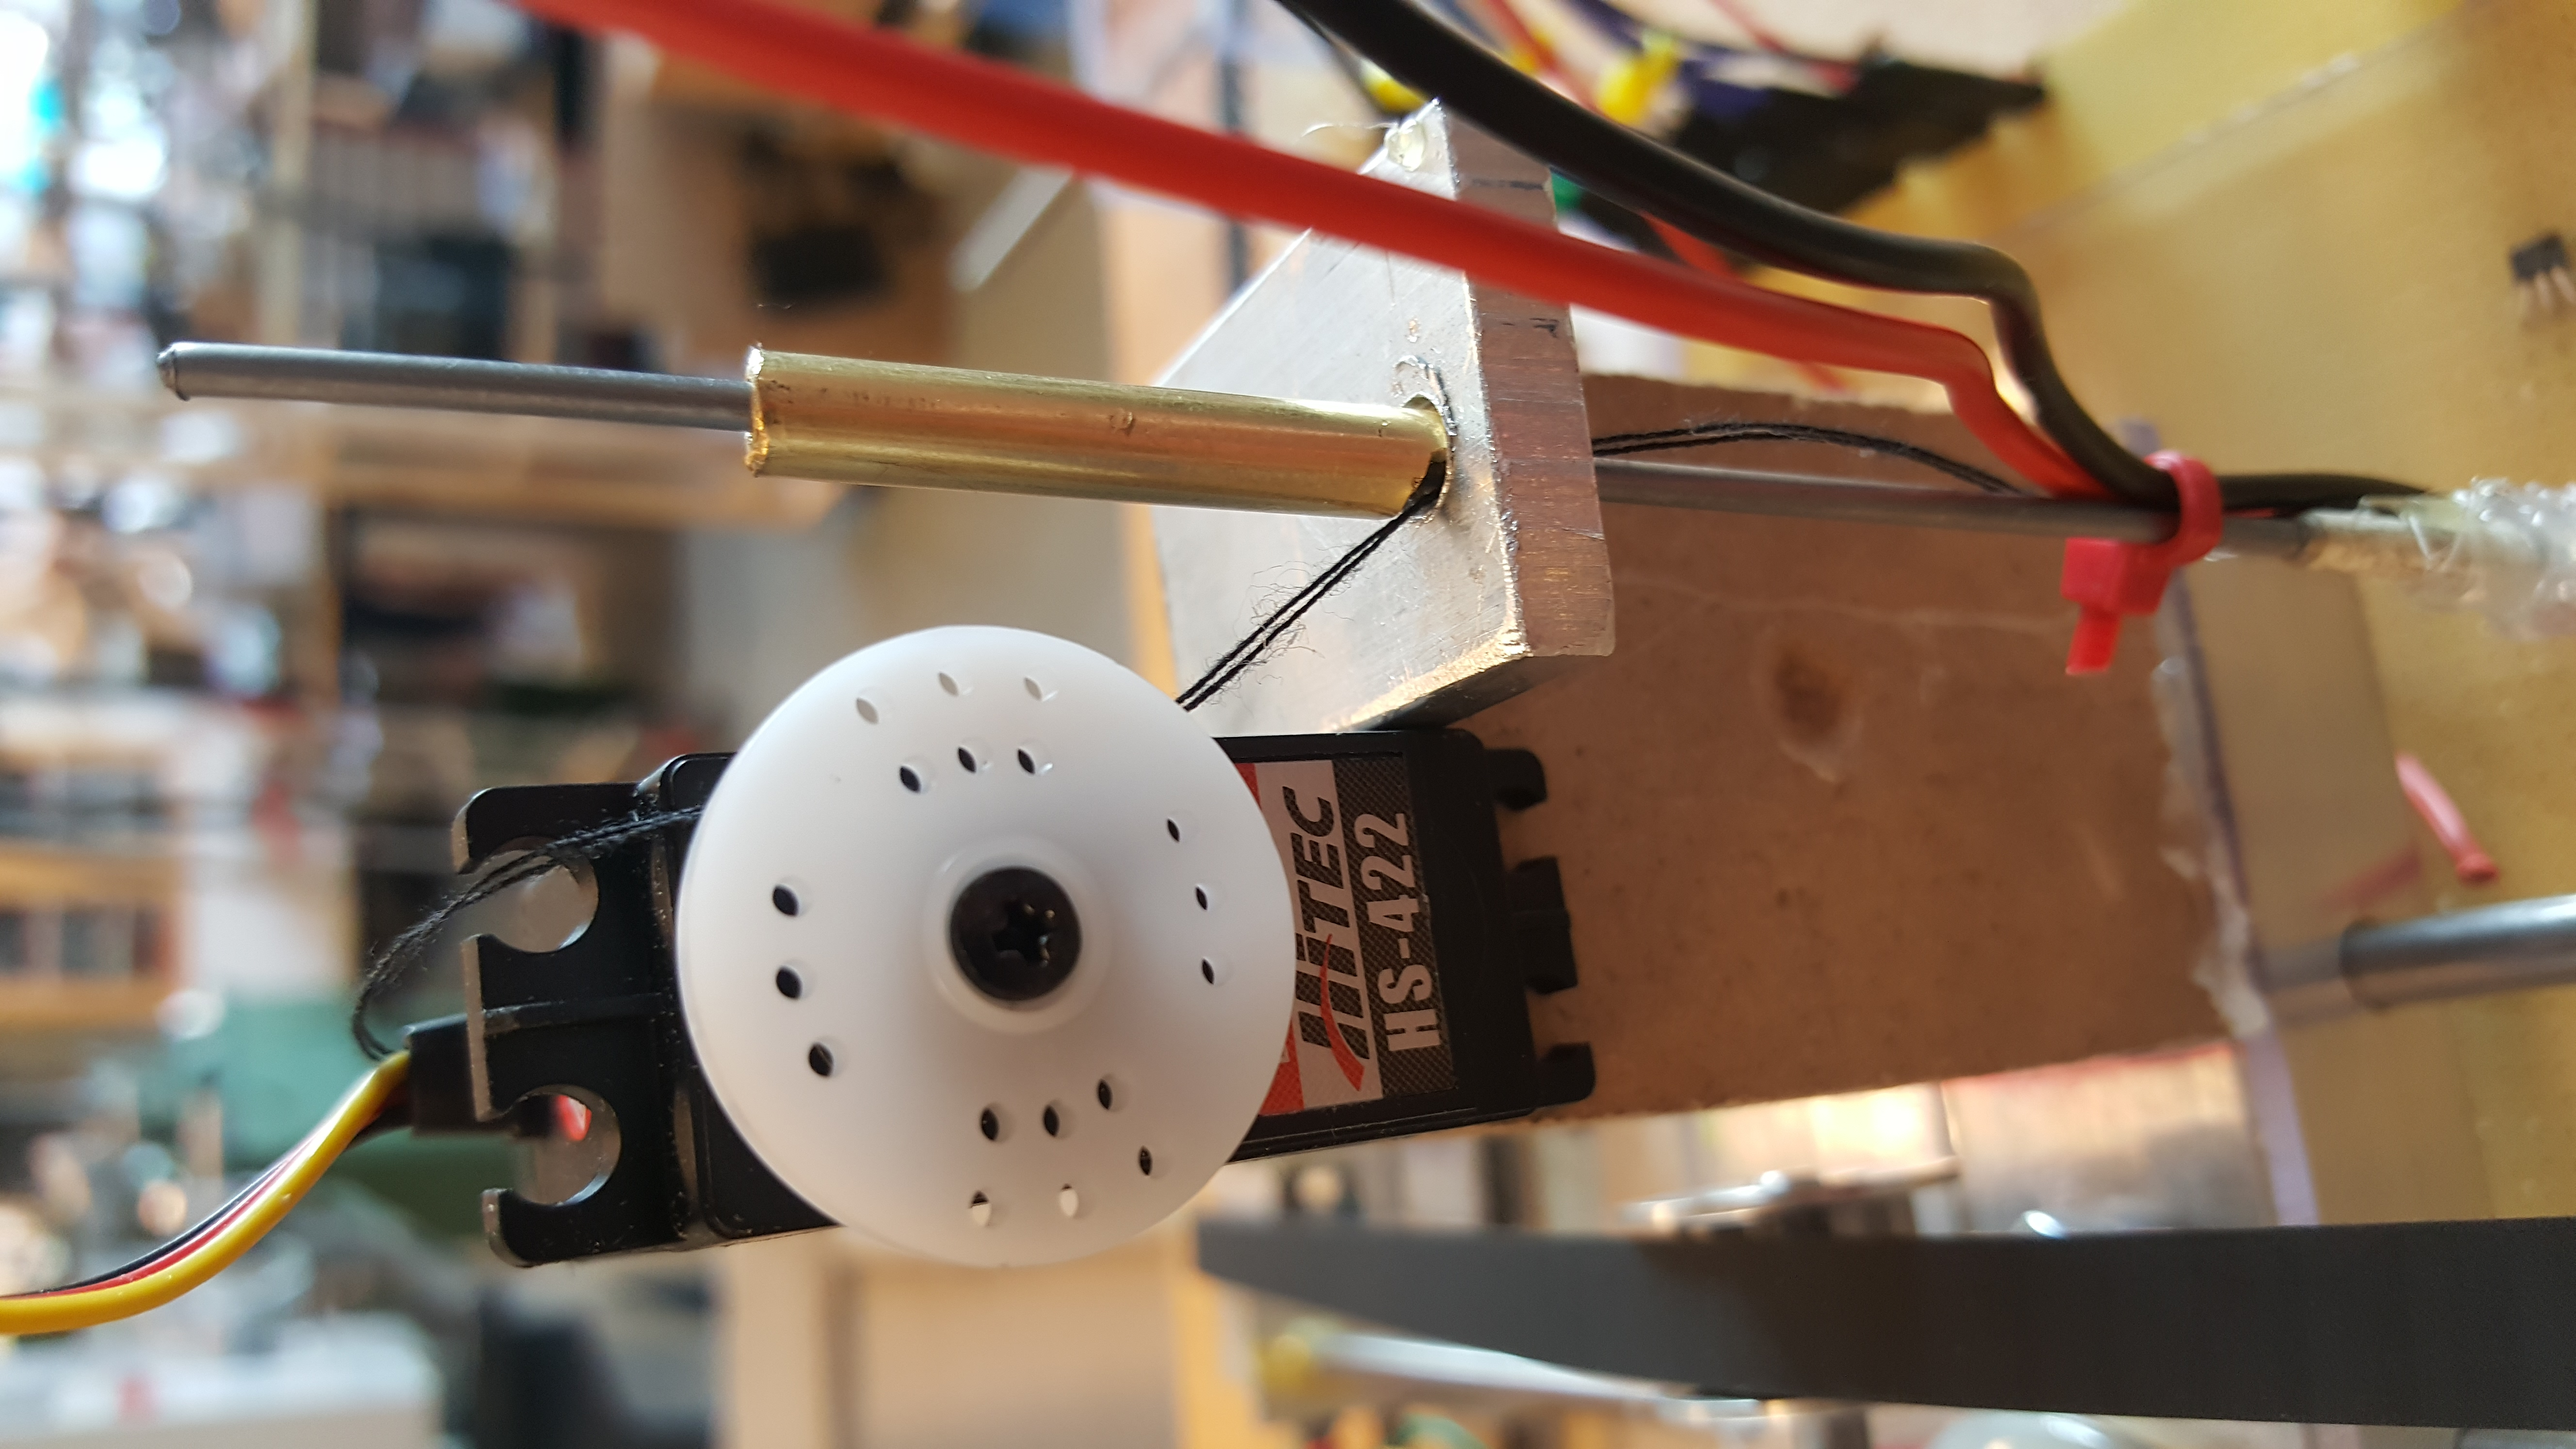
\includegraphics[width=0.4\textwidth,keepaspectratio]{../images/servo_fram}
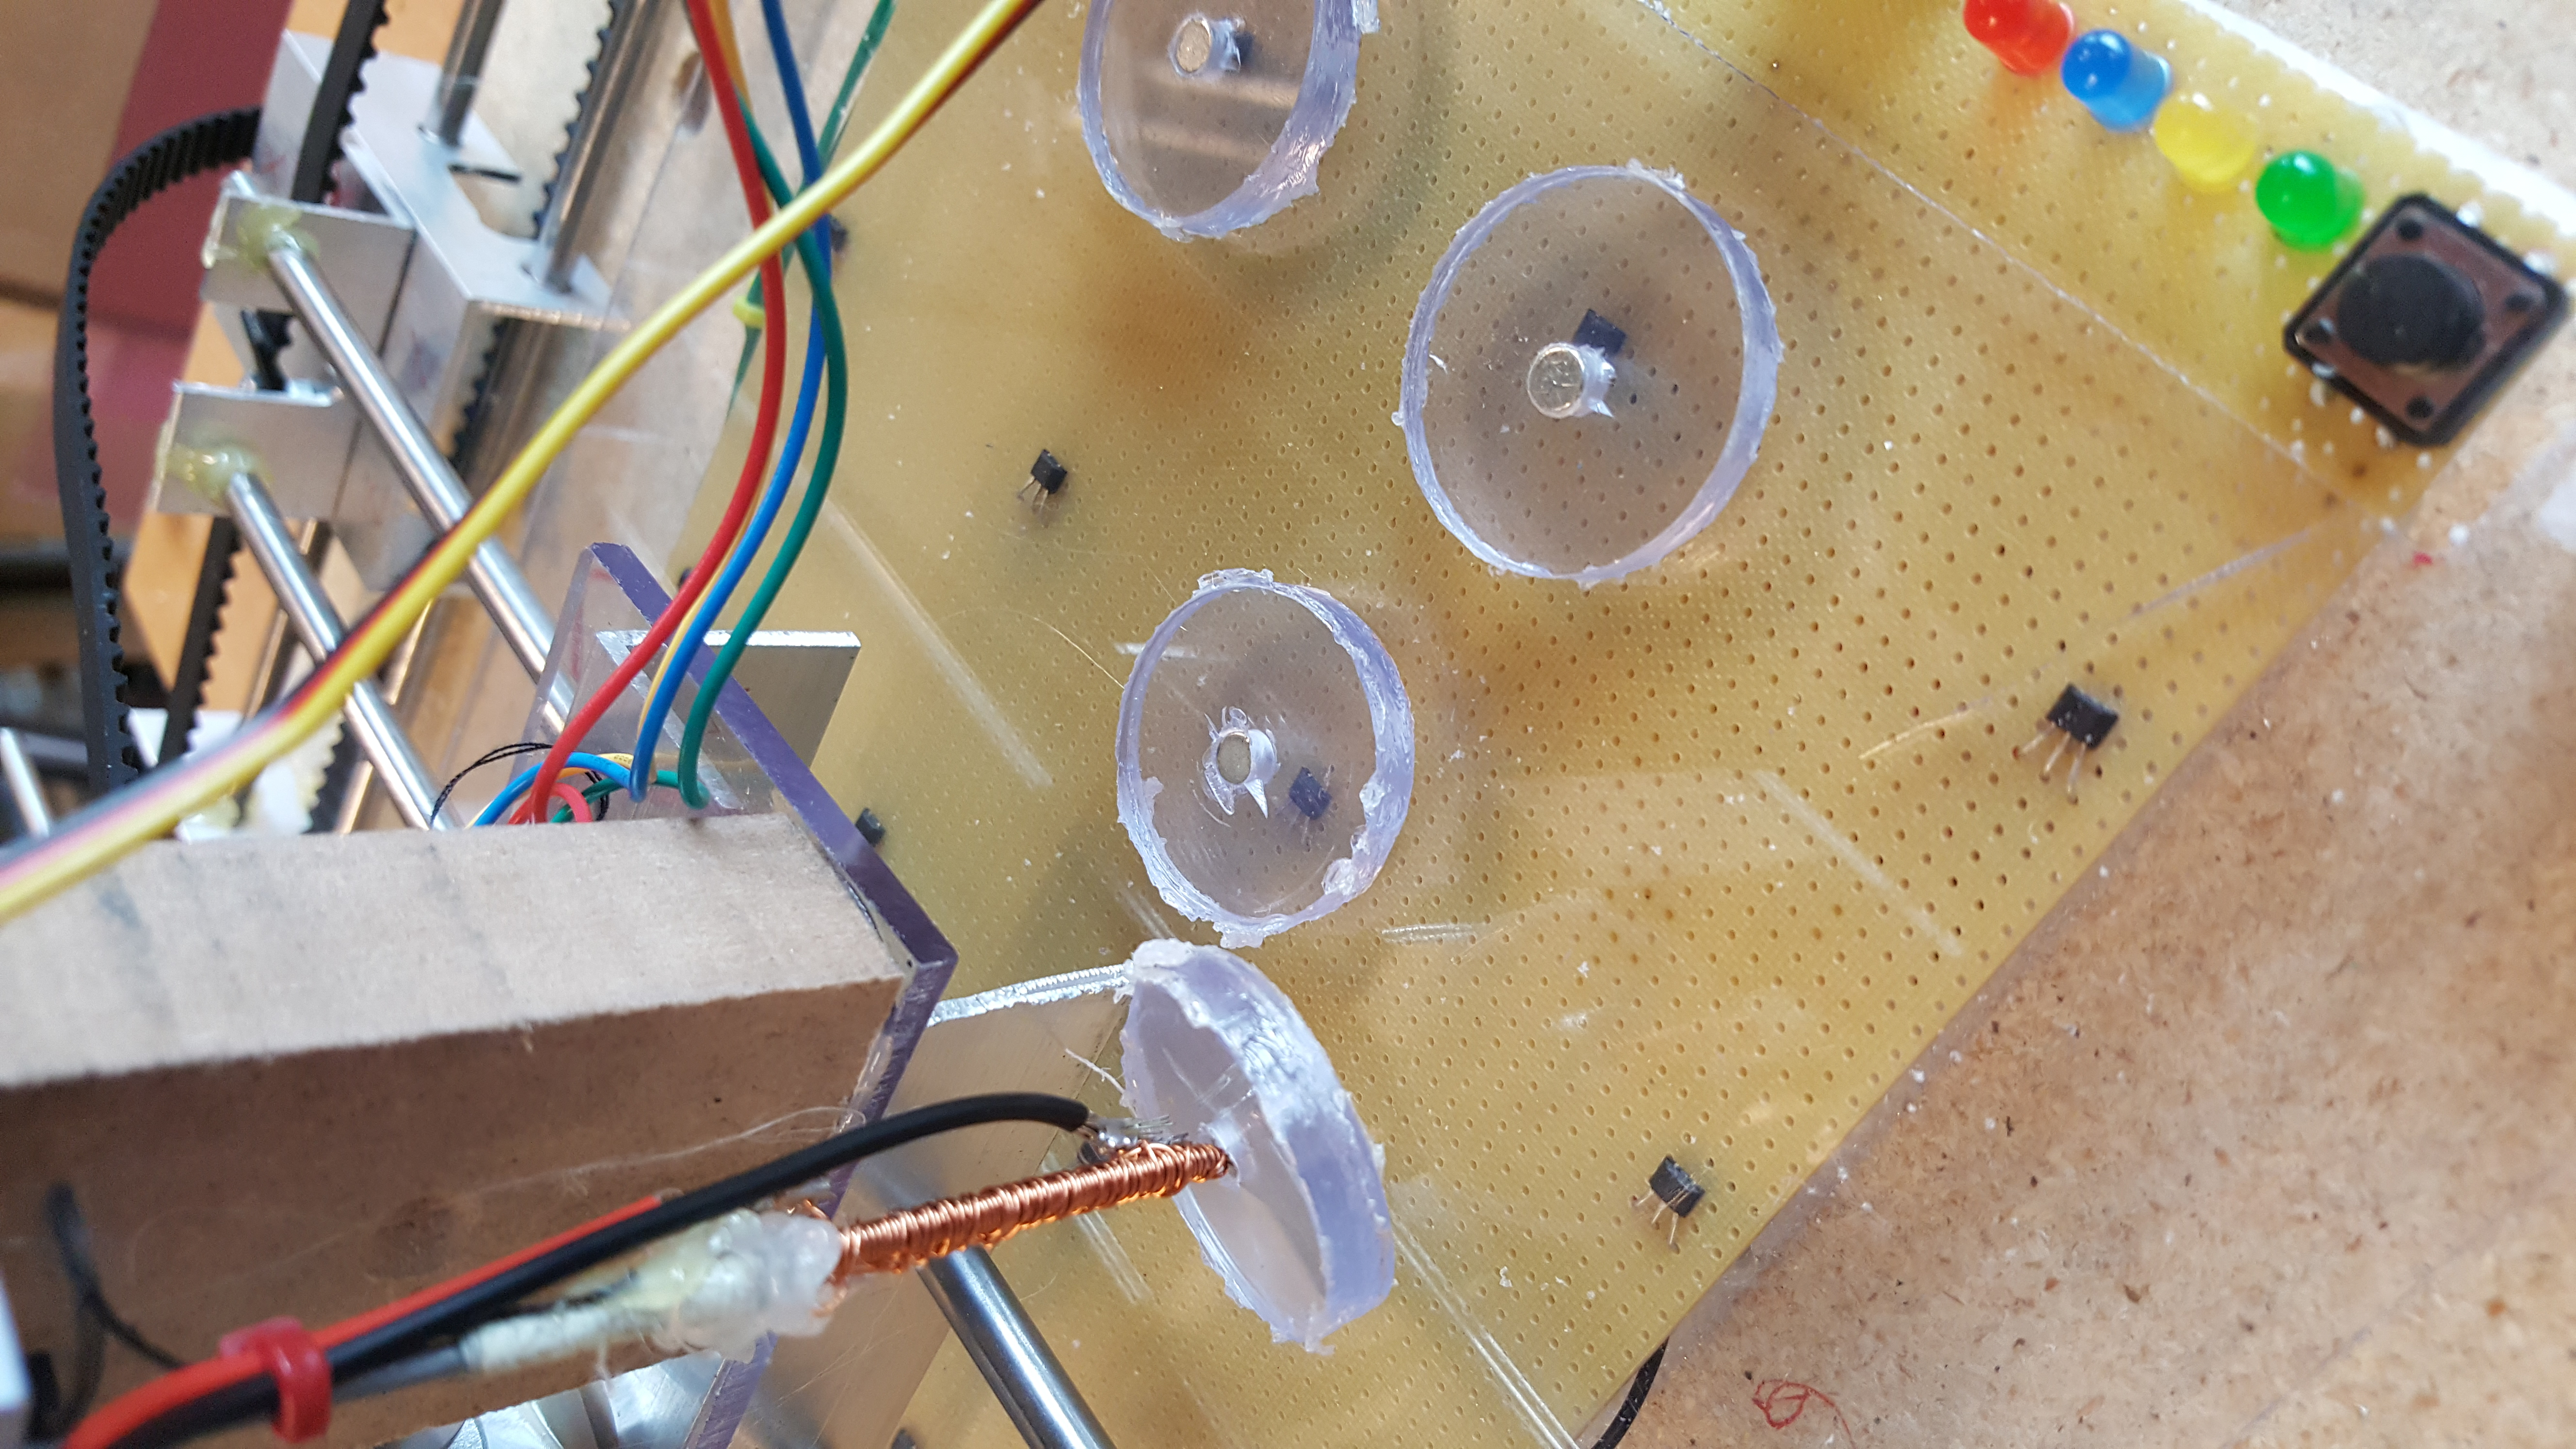
\includegraphics[width=0.4\textwidth,keepaspectratio]{../images/elektromagnet}
\caption{Vänster: Servot för höjning och sänkning av elektromagneten. Höger: Spelplan med en pjäs upplockad av elektromagneten}
\end{figure}

\subsubsection*{Spelplan och sensorer}
Spelplanen konstruerades genom att sensorerna monterades på ett kretskort i ett rutnät, se figur \ref{board}.
Kretskortet fästes sedan på undersidan av en 3mm tunn plastskiva.
Sensorerna känner av spelpjäsernas magneter linjärt men magnetfältets täthet avtar snabbt med avståndet från sensorn.
Detta gör att spelpjäsen måste placeras väldigt precist.
Om spelpjäsen placeras med mer än 1cm avvikelse från tänkt position kommer sensorn inte klara av att känna av den.
\begin{figure}\label{board}
\centering
\includegraphics[width=0.4\textwidth,keepaspectratio]{../images/spelplan_under}
\includegraphics[width=0.4\textwidth,keepaspectratio]{../images/board_top}
\caption{Vänster: Undersidan av kretskort med sensorer. Höger: Ovansida monterad under spelplanen.}
\end{figure}

\subsection{Mjukvara}


\section{Diskussion och slutsats}
Vi lyckades till viss del bygga en Othellospelande robot.
Ställningen blev klar och kunde nå cirka hälften av spelplanerna innan friktionen blev för stor och stegmotorn inte orkade med rörelsen.
Om vi skulle gjort något annorlunda hade det varit att öka precisionen så att hålen där stängerna går igenom inte fastnar.
Högre precistion skulle även möjligöra för noggrannare placering av spelpjäser.
Ett annat material än metall hade även kunnat användas vid vinkellisterna så att friktionen mellan dessa och metallplattorna minskas.
Alternativt hade även en kraftigare stegmotor kunnat utnyttjas, alternativt en strömförsörjning till stegmotorerna med högre spänning än den vi hade att tillgå och vi skulle då kunna kontrollera hela spelplanen.
\\
\\
Programmeringen med styrning och AI blev till stor del klar, dock ej testad i verkligheten eller kalibrerad.
Om man hade färdigställt hårdvaran tidigare skulle vi haft tid att kalibrera pjäskoordinaterna och därigenom kunnat köra programmet i verkligheten. 
\\
\\
Spelplanen var den del som fungerade bäst, denna kunde känna av spelpjäserna och vilken av sidorna som var uppåt.
\\
\\
Vid vidare utveckling är dessa några funktioner man skulle kunna lägga till efter grundfunktionerna fungerar: 
\begin{itemize}
    \item Möjlighet att välja färg på AI:t
    \item Efter AI:t utfört ett drag vänder den alla pjäser som blir påverkade av draget
    \item Mekanismen plockar upp nya pjäser utan mänsklig hjälp
    \item AI:n gör "smarta" drag
    \item Möjlighet att ställa in betänketid och/eller svårighetsgrad
    \item Display som kan visa mer information om state
    \item AI:t känner av när motståndaren utfört sitt drag och fortsätter automatiskt med sitt drag utan input
    \item Möjlighet att ha två olika AI:n som spelar mot varandra
    \item Bygga två stycken robotar som spelar mot varandra
\end{itemize}

\pagebreak
\begin{appendix}
\section{Källkod} \label{code}
\subsection{othello\_bot.ino}
\lstinputlisting{../../othello_bot/othello_bot.ino}
\subsection{game.hpp}
\lstinputlisting{../../othello_bot/game.hpp}
\subsection{game.cpp}
\lstinputlisting{../../othello_bot/game.cpp}
\subsection{AI.hpp}
\lstinputlisting{../../othello_bot/AI.hpp}
\subsection{AI.cpp}
\lstinputlisting{../../othello_bot/AI.cpp}
\subsection{sensor.hpp}
\lstinputlisting{../../othello_bot/sensor.hpp}
\subsection{sensor.cpp}
\lstinputlisting{../../othello_bot/sensor.cpp}
\subsection{move\_planner.hpp}
\lstinputlisting{../../othello_bot/move_planner.hpp}
\subsection{move\_planner.cpp}
\lstinputlisting{../../othello_bot/move_planner.cpp}
\subsection{IO.hpp}
\lstinputlisting{../../othello_bot/IO.hpp}
\subsection{IO.cpp}
\lstinputlisting{../../othello_bot/IO.cpp}
\subsection{config.hpp}
\lstinputlisting{../../othello_bot/config.hpp}
\subsection{random.hpp}
\lstinputlisting{../../othello_bot/random.hpp}

\section{Ritningar}
\label{sketches}
\subsection{Spelbräde}
\begin{figure}[!h]\label{board}
\centering
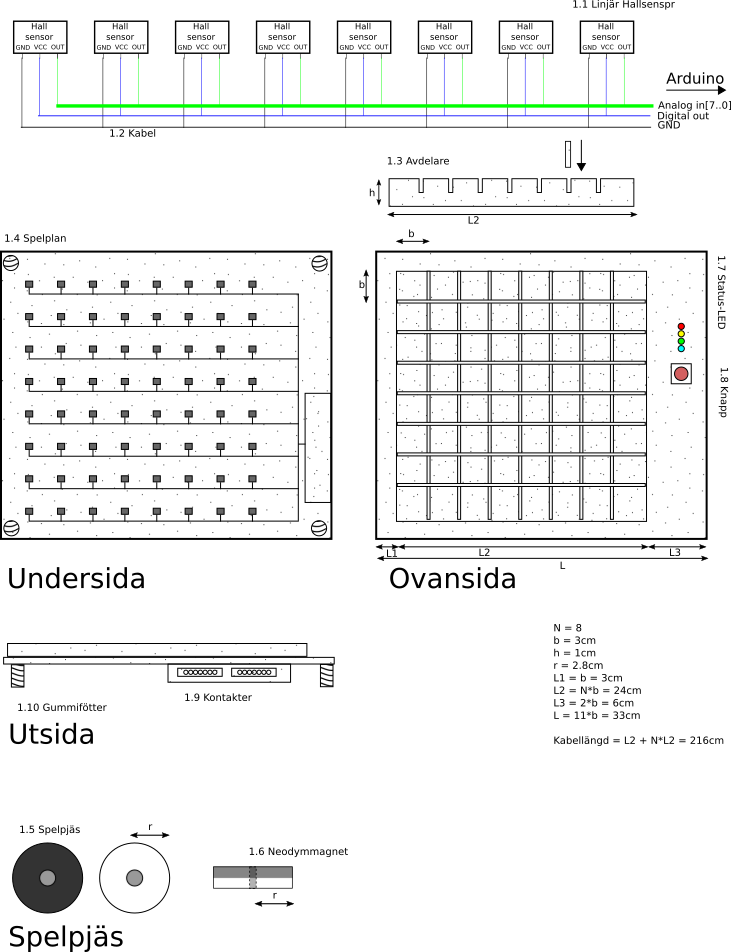
\includegraphics[scale=0.6]{board}
\caption{Ritning till spelbrädet}
\end{figure}

\subsection{Robotarm}
\begin{figure}[!h]\label{arm}
\centering
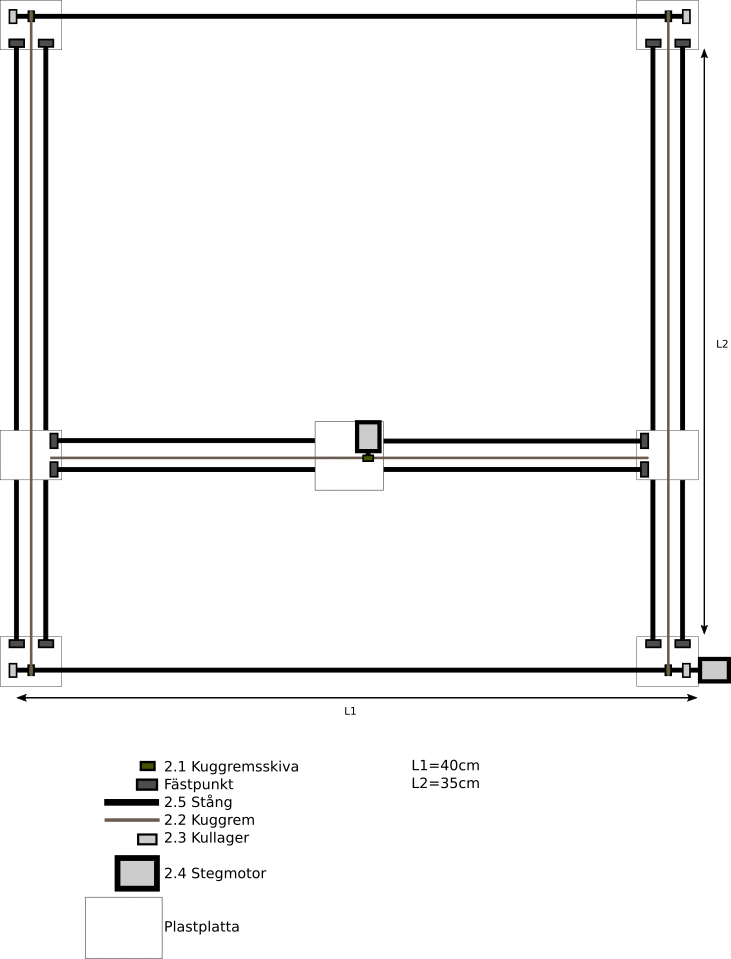
\includegraphics[scale=0.6]{arm}
\caption{Ritning till robotarmen}
\end{figure}

\section{Materiallista}
    \begin{table}
        \begin{tabular}{ | c | c | c | }
\hline
Del & Benämning & Antal/storlek \\
\hline
\hline
0.1 & Arduino Mega & 1st \\
1.1 & Linjär Halleffektsensor & 64st \\
1.2 & Kopplingskabel & 16x220cm \\
1.3 & Avdelare, plastglas & 14x24cm \\
1.4 & Plan, plastglas & 33x33cm \\
1.5 & Spelpjäs, trä & 1x45x45cm \\
1.6 & Neodymmagnet 5mmx5mm & 64st \\
1.7 & LED, 3mm grön & 4st \\
1.8 & Vippa & 1st \\
1.9 & Flatkabel, 26 poler & 0,5m \\
1.9 & Stiftlister & 2st \\
1.10 & Gummifötter & 4st \\
2.1 & Kuggremsskiva 6mm & 4st \\
2.2 & Kuggrem & 3m \\
2.3 & Kullager & 4st \\
2.4 & Stegmotor & 2st \\
2.5 & Axel 6mm & 6st \\
2.6 & Glidlager 6mm & 6st \\
2.7 & Ställning för stegmotor & 2st \\
2.8 & Stegmotordrivare & 1st \\
2.9 & Batterieliminator & 1st \\
2.10 & LCD & 1st \\
2.11 & Kuggremsskiva 5mm & 1st \\
2.12 & Plattor som fästpunkt & 4st \\
2.13 & Lim/epoxy för bland annat plast & 1st \\
3.1 & Servo & 1st \\
3.2 & Metalstav 10mm x 20cm & 1st \\
3.3 & Elektromagnet (ur relä) & 1st \\
3.4.1 & Skruv 5mm & 6st \\
3.4.2 & Mutter 5mm & 6st \\
\hline
        \end{tabular}
    \end{table}

\end{appendix}

\end{document}
